\newpage
\section{Desain dan Implementasi}

Tugas ini dilakukan sesuai dengan desain sistem berikut beserta implementasinya. Desain sistem adalah konsep dari pembuatan dan perancangan infrastruktur dan kemudian diwujudkan dalam bentuk alur yang harus dikerjakan

\subsection{Deskripsi sistem}
Pada tugas ini kita akan melakukan analisis data dan membangun model klasifikasi untuk memprediksi apakah pelanggan perusahaan telekomunikasi penyedia wifi akan berhenti berlangganan atau tidak. Dataset yang digunakan adalah dataset churn pelanggan yang berisi informasi tentang pelanggan, seperti jenis layanan, jenis kelamin, status pekerjaan, biaya langganan, dan informasi lainnya. Desain sistem ini mencakup langkah-langkah yang akan dijabarkan dalam Gambar \ref{fig:desain_sistem}.

\begin{figure}[H]
    \centering
    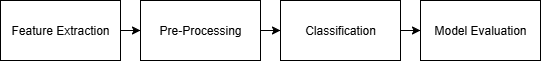
\includegraphics[width=0.8\textwidth]{gambar/metodologi.png}
    \caption{Desain Sistem}
    \label{fig:desain_sistem}
\end{figure}


\subsection{Feature Extraction}
Feature extraction adalah proses mengidentifikasi dan memilih fitur-fitur yang relevan dari dataset yang akan digunakan dalam model klasifikasi. Dalam tugas ini, fitur-fitur yang dipilih mencakup informasi tentang pelanggan, seperti jenis layanan, jenis kelamin, status pekerjaan, biaya langganan, dan informasi lainnya. 

\subsubsection{Deskripsi Fitur}
Dataset yang digunakan dalam tugas ini adalah dataset dalam format .csv yang berisi informasi langganan internet dari perusahaan telekomunikasi. Dataset ini mencakup berbagai informasi seperti customerid, jenis layanan, jenis kelamin, status pekerjaan, biaya langganan, dan informasi lainnya Setiap baris dalam dataset mewakili satu pelanggan dan setiap kolom mewakili fitur fitur tersebut. Gambar \ref{fig:dataset_customer} merupakan contoh dari dataset yang digunakan.

\begin{figure}[ht]
    \centering
    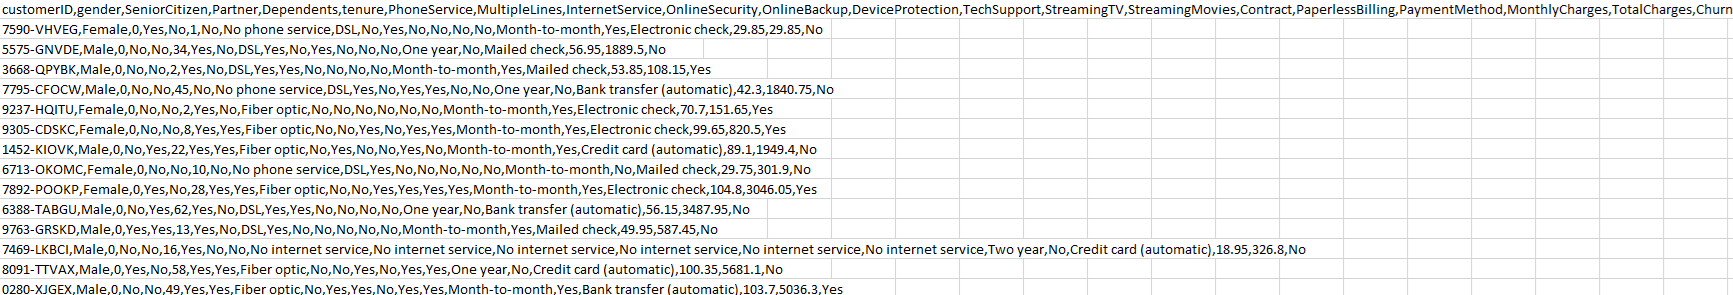
\includegraphics[width=0.8\textwidth]{gambar/dataset.png}
    \caption{Contoh Dataset Pelanggan}
    \label{fig:dataset_customer}
\end{figure}

Adapun untuk memperjelas fitur-fitur yang akan dipilih dalam metode feature selection untuk model klasifikasi kita nantinya, berikut adalah deskripsi singkat dari beberapa fitur yang terdapat dalam dataset:

% Definisi masing-masing kolom
% ● Customerid: id dari customer
% ● Gender: gender dari customer
% ● Seniorcitizen: apakah merupakan senior citizen atau tidak
% ● Partner: apakah memiliki partner atau tidak
% ● Dependents: apakah memiliki tanggungan atau tidak seperti anak dll
% ● Tenure: tenure dari langganan customer
% ● PhoneService: apakah menggunakan layanan phone atau tidak
% ● MultipleLines: apakah menggunakan multiple lines atau tidak
% ● InternetService: Tipe dari internet service yang digunakan
% ● OnlineSecurity: apakah menggunakan fitur online security
% ● OnlineBackup: apakah menggunakan fitur online backup
% ● DeviceProtection: apakah menggunakan fitur device protection
% ● TechSupport: apakah menggunakan fitur tech support atau tidak
% ● StreamingTV: apakah menggunakan fitur streaming TV atau tidak
% ● StreamingMovies: apakah menggunakan fiture streaming film atau tidak
% ● Contract: tipe contract dari customer
% ● PaperlessBilling: apakah menggunakan fitur paperless billing atau tidak
% ● PaymentMethod: payment tipe yang digunakan oleh customer
% ● MonthlyCharges: total charges/biaya bulanan yang dibayarkan
% ● TotalCharges: total charges secara keseluruhan yang dibayarkan
% ● Churn: target variabel yang menunjukan bahwa customer churn atau tidak

\begin{itemize}
    \item Customerid: ID unik dari pelanggan.
    \item Gender: Jenis kelamin pelanggan (Pria/Wanita).
    \item Seniorcitizen: Apakah pelanggan merupakan senior citizen (1 untuk ya, 0 untuk tidak).
    \item Partner: Apakah pelanggan memiliki pasangan (Ya/Tidak).
    \item Dependents: Apakah pelanggan memiliki tanggungan (Ya/Tidak).
    \item Tenure: Lama berlangganan layanan (dalam bulan).
    \item PhoneService: Apakah pelanggan menggunakan layanan telepon (Ya/Tidak).
    \item MultipleLines: Apakah pelanggan menggunakan layanan telepon multiple lines (Ya/Tidak).
    \item InternetService: Tipe layanan internet yang digunakan (DSL/Fiber optic/No).
    \item OnlineSecurity: Apakah pelanggan menggunakan fitur keamanan online (Ya/Tidak).
    \item OnlineBackup: Apakah pelanggan menggunakan fitur backup online (Ya/Tidak).
    \item DeviceProtection: Apakah pelanggan menggunakan fitur perlindungan perangkat (Ya/ Tidak).
    \item TechSupport: Apakah pelanggan menggunakan fitur dukungan teknis (Ya/Tidak).
    \item StreamingTV: Apakah pelanggan menggunakan fitur streaming TV (Ya/Tidak).
    \item StreamingMovies: Apakah pelanggan menggunakan fitur streaming film (Ya/Tidak).
    \item Contract: Tipe kontrak layanan (Month-to-month/One year/Two year).
    \item PaperlessBilling: Apakah pelanggan menggunakan penagihan tanpa kertas (Ya/Tidak).
    \item PaymentMethod: Metode pembayaran yang digunakan (Electronic check / Mailed check / Bank transfer (automatic) /Credit card (automatic)).
    \item MonthlyCharges: Biaya bulanan yang dibayarkan oleh pelanggan.
    \item TotalCharges: Total biaya yang dibayarkan oleh pelanggan selama berlangganan.
    \item Churn: Target variabel yang menunjukkan apakah pelanggan berhenti berlangganan (Ya/Tidak), dan merupakan Label target yang akan diprediksi oleh model klasifikasi.
\end{itemize}

\subsection{EDA (Exploratory Data Analysis)}
Exploratory Data Analysis (EDA) adalah proses analisis awal terhadap dataset untuk memahami struktur, pola, dan hubungan antar fitur. Dalam tugas ini, EDA dilakukan untuk mengidentifikasi karakteristik data, mendeteksi adanya missing values, outliers, dan distribusi dari setiap fitur.

Pertama tama yang kita akan lakukan adalah mengimport dataset dan menyiapkan library yang akan digunakan dalam EDA. Pandas, NumPy, Matplotlib, dan Seaborn adalah beberapa library yang umum digunakan untuk analisis data dan visualisasi di Python. Pandas digunakan untuk manipulasi data, NumPy untuk operasi numerik, Matplotlib dan Seaborn untuk visualisasi data.

\begin{lstlisting}[language=Python, caption=Import Library dan Dataset]
import pandas as pd
import numpy as np
import matplotlib.pyplot as plt
import seaborn as sns

# Import dataset
df = pd.read_csv('dataset.csv')
\end{lstlisting}

Setelah mengimport dataset, langkah selanjutnya adalah melakukan analisis awal terhadap data. Kita akan melihat beberapa informasi dasar tentang dataset, seperti jumlah baris dan kolom, tipe data dari setiap kolom, serta beberapa baris pertama dari dataset. Dengan menggunakan .info kita bisa melihat tipe data dari setiap kolom. 

\begin{lstlisting}[language=Python, caption=Informasi Awal Dataset]
# Informasi awal dataset
df.info()

# Output
<class 'pandas.core.frame.DataFrame'>
RangeIndex: 7043 entries, 0 to 7042
Data columns (total 21 columns):
 #   Column            Non-Null Count  Dtype  
---  ------            --------------  -----  
 0   customerID        7043 non-null   object 
 1   gender            7043 non-null   object 
 2   SeniorCitizen     7043 non-null   int64  
 3   Partner           7043 non-null   object 
 4   Dependents        7043 non-null   object 
 5   tenure            7043 non-null   int64  
 6   PhoneService      7043 non-null   object 
 7   MultipleLines     7043 non-null   object 
 8   InternetService   7043 non-null   object 
 9   OnlineSecurity    7043 non-null   object 
 10  OnlineBackup      7043 non-null   object 
 11  DeviceProtection  7043 non-null   object 
 12  TechSupport       7043 non-null   object 
 13  StreamingTV       7043 non-null   object 
 14  StreamingMovies   7043 non-null   object 
 15  Contract          7043 non-null   object 
 16  PaperlessBilling  7043 non-null   object 
 17  PaymentMethod     7043 non-null   object 
 18  MonthlyCharges    7043 non-null   float64
 19  TotalCharges      7043 non-null   object 
 20  Churn             7043 non-null   object 
dtypes: float64(1), int64(2), object(18)
memory usage: 1.1+ MB

\end{lstlisting}

Setelah saya analisa ternyata terdapat beberapa kolom yang memiliki tipe data yang tidak sesuai, seperti kolom TotalCharges yang seharusnya bertipe numerik namun masih bertipe object. Hal ini bisa terjadi karena adanya missing values atau karakter non-numerik dalam kolom tersebut. Oleh karena itu, kita perlu melakukan pembersihan data untuk memastikan bahwa semua kolom memiliki tipe data yang sesuai.

\begin{lstlisting}[language=Python, caption=Perbaikan Tipe Data Kolom TotalCharges]
# Mengubah tipe data kolom TotalCharges menjadi numerik
df['TotalCharges'] = pd.to_numeric(df['TotalCharges'], errors='coerce')

# Mengecek missing values setelah perubahan tipe data
missing_values = df.isnull().sum()
print("Missing values after type conversion:\n", missing_values)

# Output
customerID           0
gender               0
.....
.....
PaperlessBilling     0
PaymentMethod        0
MonthlyCharges       0
TotalCharges        11
Churn                0
dtype: int64
\end{lstlisting}

Saya juga melakukan pengecekan terhadap missing values pada dataset. Dengan menggunakan .isnull().sum() kita bisa melihat jumlah missing values pada setiap kolom. Dari hasil pengecekan, terdapat 11 missing values pada kolom TotalCharges. Kita perlu menangani missing values ini sebelum melanjutkan analisis lebih lanjut.

Untuk menangani missing values pada kolom TotalCharges, kita bisa menghapus baris yang memiliki missing values tersebut atau mengisi missing values dengan nilai rata-rata atau median dari kolom tersebut. Dalam tugas ini, saya memilih untuk menghapus baris yang memiliki missing values.

\newpage

\begin{lstlisting}[language=Python, caption=Menghapus Missing Values]
# output
.....
.....
MonthlyCharges      0
TotalCharges        0
Churn               0
dtype: int64
\end{lstlisting}

Kita telah selesai menghapus missing values pada kolom TotalCharges. Setelah itu, kita akan melakukan analisis lebih lanjut terhadap fitur-fitur yang ada dalam dataset. Kita akan melihat distribusi dari setiap fitur, hubungan antar fitur, serta outliers yang mungkin ada dalam dataset.

Agar memudahkan analisa maka dataset akan dibagi menjadi dua bagian, yaitu dataset untuk fitur numerik dan dataset untuk fitur kategorikal. Hal ini dilakukan agar analisis dapat dilakukan dengan lebih efektif.

Adapun pembagiannya sebagai berikut :
\begin{lstlisting}[language=Python, caption=Memisahkan Fitur Numerik dan Kategorikal]
    Numerical Columns: ['tenure', 'MonthlyCharges', 'TotalCharges']
    Categorical Columns: ['customerID', 'gender', 'SeniorCitizen', 
    'Partner', 'Dependents', 'PhoneService', 'MultipleLines', 
    'InternetService', 'OnlineSecurity', 'OnlineBackup', 
    'DeviceProtection', 'TechSupport', 'StreamingTV', 
    'StreamingMovies', 'Contract', 'PaperlessBilling', 
    'PaymentMethod', 'Churn']
\end{lstlisting}

\subsubsection{Analisis Fitur Kategorikal}
Analisis fitur kategorikal dilakukan untuk memahami distribusi dari setiap fitur kategorikal dalam dataset. Kita akan menggunakan visualisasi seperti bar plot untuk melihat jumlah pelanggan berdasarkan setiap kategori. Namun agar barplot tidak terlalu banyak kita akan uji dengan chi square terlebih dahulu untuk melihat fitur mana saja yang signifikan terhadap target variabel Churn. Dengan begitu kita bisa plot barplot hanya untuk fitur yang signifikan saja.



% Berikut hasil uji chi square, buatkan tabel perangkingan dari hasil ini beserta outputnya
% InternetService : Chi-squared: 728.6956143058694, p-value: 5.831198962237274e-159, degrees of freedom: 2. There is a significant association between Internet Service and Churn. Cramer's V: 0.3219093912684771
% Gender: Chi-squared: 0.47545453727386294, p-value: 0.490488470706551, degrees of freedom: 1. There is no significant association between Gender and Churn. Cramer's V: 0.008222711767086818
% SeniorCitizen : Chi-squared: 158.4408162893713, p-value: 2.4792557203954705e-36, degrees of freedom: 1 There is a significant association between Senior Citizen and Churn. Cramer's V: 0.15010463561752393
% Partner : Chi-squared: 157.50315146557506, p-value: 3.97379757451591e-36, degrees of freedom: 1 There is a significant association between Partner and Churn. Cramer's V: 0.1496598111790044
% Dependents : Chi-squared: 186.32163933855873, p-value: 2.0196592017051303e-42, degrees of freedom: 1. There is a significant association between Dependents and Churn. Cramer's V: 0.16277669159928557
% PhoneService : Chi-squared: 0.8737327674431736, p-value: 0.34992398942431924, degrees of freedom: 1. There is no significant association between Phone Service and Churn. Cramer's V: 0.011146791573280324
% MultipleLines : Chi-squared: 11.271540824020612, p-value: 0.0035679273999811405, degrees of freedom: 2. There is a significant association between Multiple Lines and Churn. Cramer's V: 0.040036141280711854
% OnlineSecurity : Chi-squared: 846.6773889208487, p-value: 1.4006867477839222e-184, degrees of freedom: 2. There is a significant association between Online Security and Churn. Cramer's V: 0.3469920701082114
% OnlineBackup : Chi-squared: 599.1751847059026, p-value: 7.776099238804965e-131, degrees of freedom: 2. There is a significant association between Online Backup and Churn. Cramer's V: 0.291902273936468
% DeviceProtection : Chi-squared: 555.8803273428508, p-value: 1.9593887862403176e-121, degrees of freedom: 2 . There is a significant association between Device Protection and Churn. Cramer's V: 0.28115850233148504
% TechSupport : Chi-squared: 824.925564387502, p-value: 7.407807748843711e-180, degrees of freedom: 2. There is a significant association between Tech Support and Churn. Cramer's V: 0.342505815780552
% StreamingTV : Chi-squared: 372.4565019355074, p-value: 1.324641113169159e-81, degrees of freedom: 2. There is a significant association between Streaming TV and Churn. Cramer's V: 0.23014330684583634
% StreamingMovies : Chi-squared: 374.2684315732459, p-value: 5.353560421401324e-82, degrees of freedom: 2. There is a significant association between Streaming Movies and Churn. Cramer's V: 0.23070242924775253
% PaperlessBilling : Chi-squared: 256.87490836218717, p-value: 8.236203353962564e-58, degrees of freedom: 1. There is a significant association between Paperless Billing and Churn. Cramer's V: 0.19112672191120977
% PaymentMethod : Chi-squared: 645.4299001234638, p-value: 1.4263098511063342e-139, degrees of freedom: 3. There is a significant association between Payment Method and Churn. Cramer's V: 0.30295987245491557
% Contract : Chi-squared: 1179.5458287339445, p-value: 7.326182186265472e-257, degrees of freedom: 2 There is a significant association between Contract and Churn. Cramer's V: 0.4095604189089921

%buatkan tabel dari data diatas dengan kolom nama_fitur, chi_squared, p_value, significant_association, cramer_v

Setelah melakukan pengecekan menggunakan chi-square saya menemukan bahwa terdapat fitur fitur yang signifikan terhadap target variabel Churn. Adapun Tabel \ref{tabel_uji}berikut adalah hasil dari uji chi-square yang dilakukan.

\begin{table}[H]
    \centering
    \caption{Hasil Uji Chi-Square}
    \label{tabel_uji}
    \begin{tabular}{|l|l|l|l|l|}
        \hline
        \textbf{Nama Fitur} & \textbf{Chi-Squared} & \textbf{P-Value} & \textbf{Significant Association} & \textbf{Cramer's V} \\ \hline
        Contract & 1179.55 & $7.33 \times 10^{-257}$ & Ya & 0.4096 \\ \hline
        TechSupport & 824.93 & $7.41 \times 10^{-180}$ & Ya & 0.3425 \\ \hline
        OnlineSecurity & 846.68 & $1.40 \times 10^{-184}$ & Ya & 0.3470 \\ \hline
        InternetService & 728.70 & $5.83 \times 10^{-159}$ & Ya & 0.3219 \\ \hline
        PaymentMethod & 645.43 & $1.43 \times 10^{-139}$ & Ya & 0.3030 \\ \hline
        OnlineBackup & 599.18 & $7.78 \times 10^{-131}$ & Ya & 0.2919 \\ \hline
        DeviceProtection & 555.88 & $1.96 \times 10^{-121}$ & Ya & 0.2812 \\ \hline
        StreamingMovies & 374.27 & $5.35 \times 10^{-82}$ & Ya & 0.2307 \\ \hline
        StreamingTV & 372.46 & $1.32 \times 10^{-81}$ & Ya & 0.2301 \\ \hline
        Dependents & 186.32 & $2.02 \times 10^{-42}$ & Ya & 0.1628 \\ \hline
        SeniorCitizen & 158.44 & $2.48 \times 10^{-36}$ & Ya & 0.1501 \\ \hline
        Partner & 157.50 & $3.97 \times 10^{-36}$ & Ya & 0.1497 \\ \hline
        MultipleLines & 11.27 & 0.0036 & Ya & 0.0400 \\ \hline
        PhoneService & 0.87 & 0.35 & Tidak & 0.0111 \\ \hline
        Gender & 0.48 & 0.49 & Tidak & 0.0082 \\ \hline

    \end{tabular}
\end{table}

Dapat dilihat bahwa fitur yang memiliki nilai Chi-Squared yang tinggi dan p-value yang sangat kecil menunjukkan adanya hubungan yang signifikan dengan target variabel Churn. Fitur-fitur seperti Contract, TechSupport, OnlineSecurity, dan InternetService memiliki nilai Cramer's V yang cukup tinggi, menunjukkan bahwa fitur-fitur tersebut memiliki pengaruh yang signifikan terhadap keputusan pelanggan untuk berhenti berlangganan.

Sedangkan fitur dengan nilai Chi-Squared yang rendah dan p-value yang tinggi menunjukan kebalikannya yaitu tidak ada hubungan yang signifikan terhadap label target variabel churn. Fitur-fitur seperti PhoneService dan Gender tidak menunjukkan hubungan yang signifikan dengan target variabel Churn, sehingga kita tidak perlu melakukan analisis lebih lanjut terhadap fitur-fitur tersebut. 

Setelah mengetahui fitur-fitur yang signifikan, kita akan melakukan visualisasi untuk melihat distribusi dari setiap fitur kategorikal yang signifikan terhadap target variabel Churn. Kita akan menggunakan bar plot untuk melihat jumlah pelanggan berdasarkan setiap kategori.

Adapun pertanyaan yang ingin saya jawab untuk analisis fitur kategorikal ini adalah sebagai berikut:
\begin{itemize}
    \item Apakah pelanggan yang dengan contract kerja tertentu cendrung churn?
    \item Apakah pelanggan yang memilih langganan dengan paket bantuan TechSupport cendrung churn?
    \item Apakah pelanggan yang memilih layanan keamanan online cendrung churn?
    \item Apakah pelanggan yang memilih layanan internet tertentu cendrung churn?
    \item Apakah pelanggan yang memilih metode pembayaran tertentu cendrung churn?
\end{itemize}

Untuk menjawab pertanyaan pertama yaitu apakah pelanggan yang dengan contract kerja tertentu cenderung churn, kita akan membuat bar plot untuk melihat jumlah pelanggan berdasarkan jenis kontrak. Kita akan membandingkan jumlah pelanggan yang churn dan tidak churn berdasarkan jenis kontrak. Dengan menggunakan .barplot() dari Seaborn, kita bisa membuat visualisasi yang jelas dan mudah dipahami. Gambar \ref{fig:contract_churn} menunjukkan hasil dari visualisasi tersebut.

\begin{figure}[H]
    \centering
    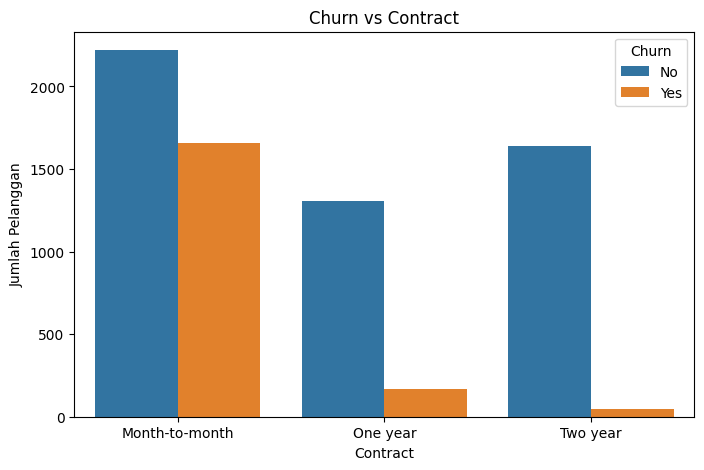
\includegraphics[width=0.8\textwidth]{gambar/contract.png}
    \caption{Jumlah Pelanggan Churn Berdasarkan Jenis Kontrak}
    \label{fig:contract_churn}
\end{figure}

Dari Gambar \ref{fig:contract_churn} dapat dilihat bahwa pelanggan dengan kontrak "Month-to-month" memiliki jumlah churn yang paling tinggi dibandingkan dengan kontrak "One year" dan "Two year". Hal ini menunjukkan bahwa pelanggan yang memilih kontrak bulanan cenderung lebih sering berhenti berlangganan dibandingkan dengan pelanggan yang memilih kontrak tahunan atau dua tahunan.

Untuk pertanyaan kedua yaitu apakah pelanggan yang memilih langganan dengan paket bantuan TechSupport cenderung churn, kita akan membuat bar plot untuk melihat jumlah pelanggan berdasarkan pilihan TechSupport. Kita akan membandingkan jumlah pelanggan yang churn dan tidak churn berdasarkan pilihan TechSupport. Gambar \ref{fig:techsupport_churn} menunjukkan hasil dari visualisasi tersebut.

\begin{figure}[H]
    \centering
    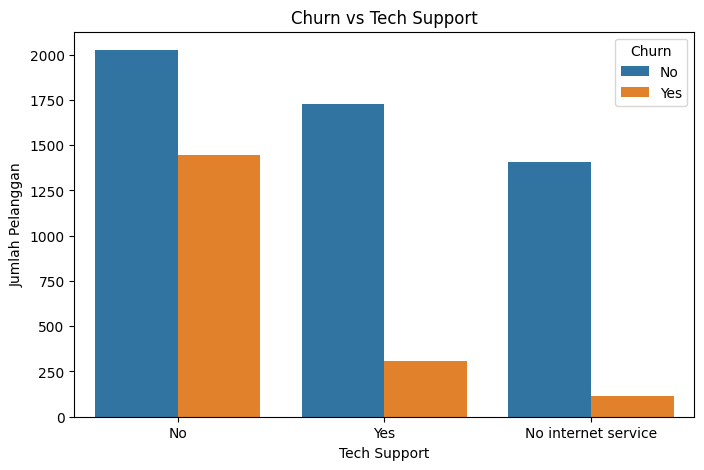
\includegraphics[width=0.8\textwidth]{gambar/techsupport.png}
    \caption{Jumlah Pelanggan Churn Berdasarkan Pilihan TechSupport}
    \label{fig:techsupport_churn}
\end{figure}

Dari Gambar \ref{fig:techsupport_churn} dapat dilihat bahwa pelanggan yang memilih untuk menggunakan layanan TechSupport memiliki jumlah churn yang lebih rendah dibandingkan dengan pelanggan yang tidak menggunakan layanan TechSupport. Hal ini menunjukkan bahwa layanan TechSupport dapat membantu mengurangi tingkat churn pelanggan.

Untuk pertanyaan ketiga yaitu apakah pelanggan yang memilih layanan keamanan online cenderung churn, kita akan membuat bar plot untuk melihat jumlah pelanggan berdasarkan pilihan OnlineSecurity. Kita akan membandingkan jumlah pelanggan yang churn dan tidak churn berdasarkan pilihan OnlineSecurity. Gambar \ref{fig:onlinesecurity_churn} menunjukkan hasil dari visualisasi tersebut.

\begin{figure}[H]
    \centering
    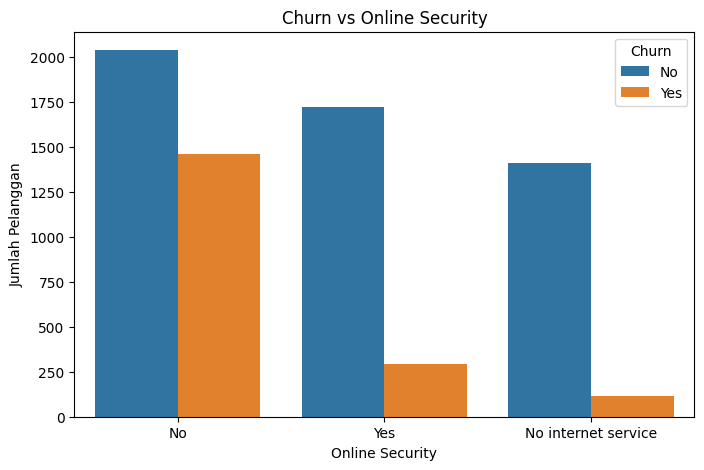
\includegraphics[width=0.8\textwidth]{gambar/onlinesecurity.png}
    \caption{Jumlah Pelanggan Churn Berdasarkan Pilihan OnlineSecurity}
    \label{fig:onlinesecurity_churn}
\end{figure}

Dari Gambar \ref{fig:onlinesecurity_churn} dapat dilihat bahwa pelanggan yang memilih untuk menggunakan layanan OnlineSecurity memiliki jumlah churn yang lebih rendah dibandingkan dengan pelanggan yang tidak menggunakan layanan OnlineSecurity. Hal ini menunjukkan bahwa layanan OnlineSecurity dapat membantu mengurangi tingkat churn pelanggan.

Untuk pertanyaan keempat yaitu apakah pelanggan yang memilih layanan internet tertentu cenderung churn, kita akan membuat bar plot untuk melihat jumlah pelanggan berda sarkan jenis layanan internet. Kita akan membandingkan jumlah pelanggan yang churn dan tidak churn berdasarkan jenis layanan internet. Gambar \ref{fig:internetservice_churn} menunjukkan hasil dari visualisasi tersebut.

\begin{figure}[H]
    \centering
    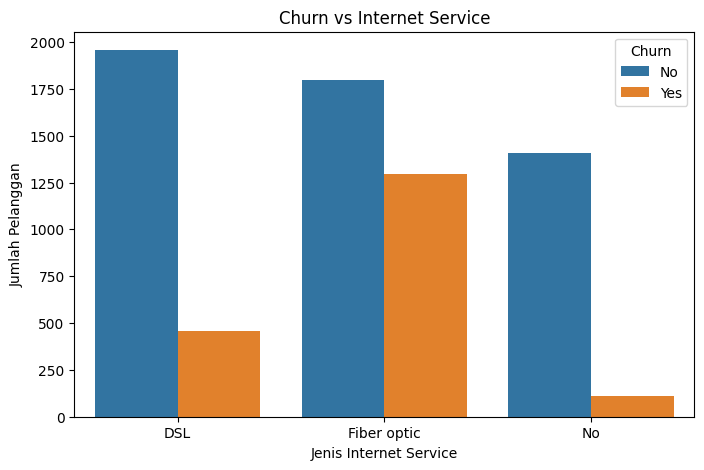
\includegraphics[width=0.8\textwidth]{gambar/internetservice.png}
    \caption{Jumlah Pelanggan Churn Berdasarkan Jenis Layanan Internet}
    \label{fig:internetservice_churn}
\end{figure}

Dari Gambar \ref{fig:internetservice_churn} dapat dilihat bahwa pelanggan yang menggunakan layanan internet "Fiber optic" memiliki jumlah churn yang paling tinggi dibandingkan dengan pelanggan yang menggunakan layanan "DSL" atau "No". Hal ini menunjukkan bahwa pelanggan yang menggunakan layanan internet Fiber optic cenderung lebih sering berhenti berlangganan dibandingkan dengan pelanggan yang menggunakan layanan DSL atau tidak menggunakan layanan internet.

Untuk pertanyaan terakhir yaitu apakah pelanggan yang memilih metode pembayaran tertentu cenderung churn, kita akan membuat bar plot untuk melihat jumlah pelanggan berdasarkan metode pembayaran. Kita akan membandingkan jumlah pelanggan yang churn dan tidak churn berdasarkan metode pembayaran. Gambar \ref{fig:paymentmethod_churn} menunjukkan hasil dari visualisasi tersebut.

\begin{figure}[H]
    \centering
    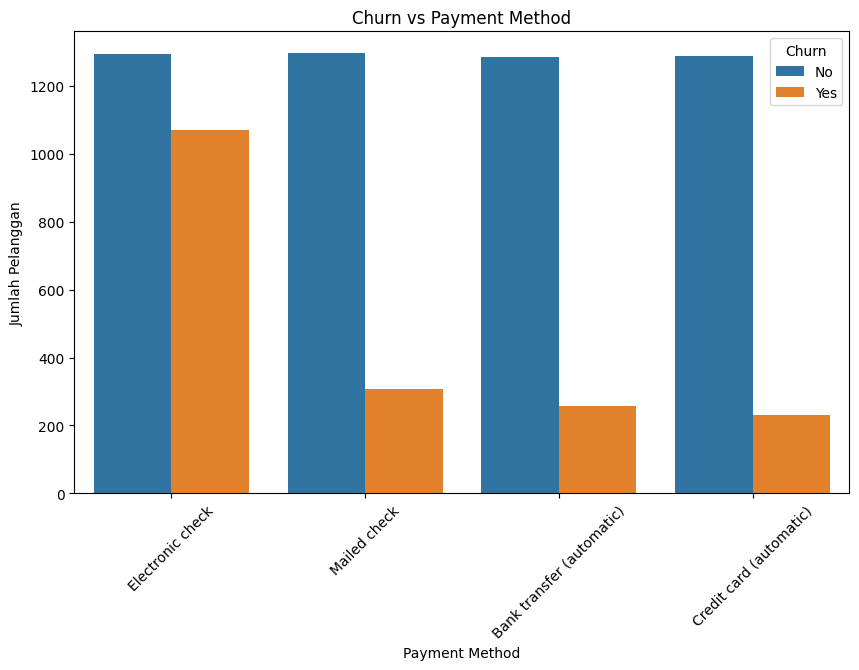
\includegraphics[width=0.8\textwidth]{gambar/paymentmethod.png}
    \caption{Jumlah Pelanggan Churn Berdasarkan Metode Pembayaran}
    \label{fig:paymentmethod_churn}
\end{figure}

Dari Gambar \ref{fig:paymentmethod_churn} dapat dilihat bahwa pelanggan yang menggunakan metode pembayaran "Electronic check" memiliki jumlah churn yang paling tinggi dibandingkan dengan metode pembayaran lainnya. Hal ini menunjukkan bahwa pelanggan yang menggunakan metode pembayaran Electronic check cenderung lebih sering berhenti berlangganan dibandingkan dengan pelanggan yang menggunakan metode pembayaran lainnya.

Dari hasil analisa diatas kita tidak hanya mendapatkan fitur yang relevan dalam membangun model klasifikasi, tetapi juga mendapatkan insight bisnis yang dapat digunakan untuk meningkatkan retensi pelanggan. Adapun insight yang didapatkan dari analisis fitur kategorikal ini adalah sebagai berikut:

\begin{itemize}
    \item Pelanggan dengan kontrak "Month-to-month" cenderung lebih sering berhenti berlangganan dibandingkan dengan pelanggan yang bekerja dengan kontrak tahunan atau dua tahunan.
    \item Layanan TechSupport dapat membantu mengurangi tingkat churn pelanggan.
    \item Layanan OnlineSecurity dapat membantu mengurangi tingkat churn pelanggan.
    \item Pelanggan yang menggunakan layanan internet "Fiber optic" cenderung lebih sering berhenti berlangganan dibandingkan dengan pelanggan yang menggunakan layanan DSL atau tidak menggunakan layanan internet.
    \item Pelanggan yang menggunakan metode pembayaran "Electronic check" cenderung lebih sering berhenti berlangganan dibandingkan dengan pelanggan yang menggunakan metode pembayaran lainnya.
\end{itemize}

Sehingga kita bisa membuat keputusan bisnis yang lebih baik berdasarkan hasil analisis ini. Adapun implikasi bisnisnya dari insight yang dihasilkan adalah sebagai berikut:

\begin{itemize}
    \item Perusahaan dapat meningkatkan layanan TechSupport untuk membantu mengurangi tingkat churn pelanggan.
    \item Perusahaan dapat meningkatkan layanan OnlineSecurity untuk membantu mengurangi tingkat churn pelanggan.
    \item Perusahaan dapat mempertimbangkan untuk meningkatkan kualitas layanan internet Fiber optic untuk mengurangi tingkat churn pelanggan. Ataupun mengurangi biaya langganan untuk pelanggan yang menggunakan layanan internet Fiber optic.
    \item Perusahaan dapat mempertimbangkan untuk menawarkan metode pembayaran yang lebih fleksibel kepada pelanggan yang menggunakan metode pembayaran Electronic check.
    \item Perusahaan dapat melakukan penawaran khusus atau promosi untuk pelanggan yang masih bekerja dengan kontrak "Month-to-month" untuk meningkatkan retensi pelanggan.
\end{itemize}

Selain insight dan implikasi bisnis diatas, kita juga dapat ditur yang relevan untuk digunakan pada feature selection pada model klasifikasi kita nantinya. Namun sebelumnya kita juga perlu tahu korelasi antar fitur kategorikal ini agar kita mengetahui fitur fitur apa saja yang redundant, Adapun kita akan menggunakan Cramer V yang sudah kita dapatkan tadi untuk menghitung korelasi antar fitur kategorikal. Cramer V adalah ukuran asosiasi antara dua variabel kategorikal yang berkisar antara 0 (tidak ada asosiasi) hingga 1 (asosiasi sempurna). Kita akan membuat matriks korelasi menggunakan Cramer V untuk melihat hubungan antar fitur kategorikal. Gambar \ref{fig:cramervheatmap} menunjukkan hasil dari heatmap korelasi Cramer V antar fitur Kategorikal.

\begin{figure}[H]
    \centering
    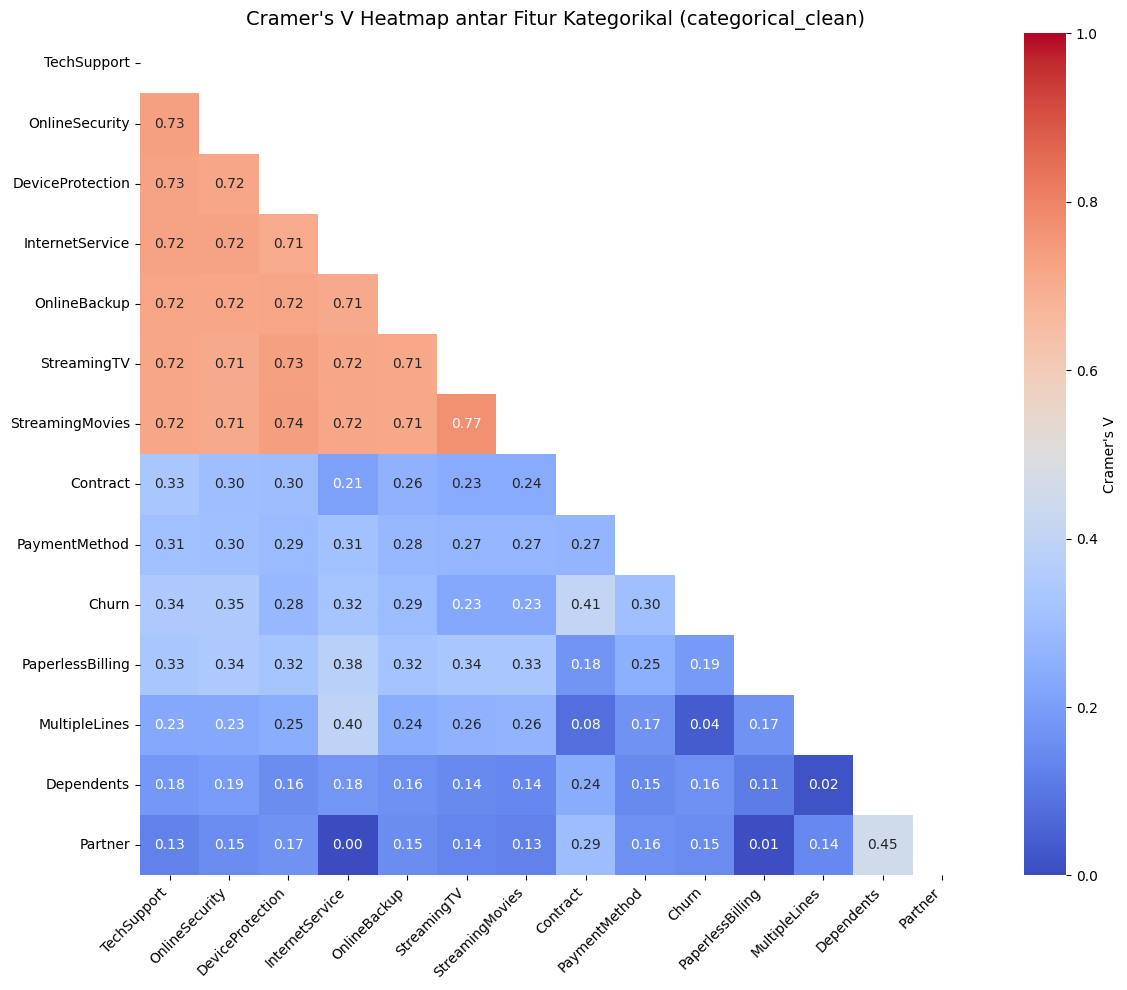
\includegraphics[width=0.8\textwidth]{gambar/cramerheatmap.png}
    \caption{Heatmap Korelasi Cramer V Antar Fitur Kategorikal}
    \label{fig:cramervheatmap}
\end{figure}

Dari Gambar \ref{fig:cramervheatmap} dapat dilihat bahwa terdapat beberapa fitur yang memiliki korelasi tinggi ditandai dengan warna yang lebih merah. Dan fitur fitur yang memiliki korelasi rendah ditandai dengan warna yang lebih biru. Adapun dengan temuan ini kita bisa melakukan feature selection untuk memilih fitur-fitur yang relevan dan tidak redundant. Kita akan memilih fitur-fitur yang memiliki korelasi tinggi dengan target variabel Churn dan menghindari fitur-fitur yang memiliki korelasi tinggi satu sama lain.

\subsubsection{Analisis Fitur Numerik}
Analisis fitur numerik dilakukan untuk memahami distribusi dari setiap fitur numerik dalam dataset. Kita akan menggunakan visualisasi seperti histogram, lalu melihat heatmap korelasi untuk melihat hubungan antar fitur numerik. Kita juga akan melakukan analisis statistik untuk melihat apakah terdapat outliers pada fitur-fitur numerik.

Pertama-tama, kita akan melihat ukuran pemusatan dari setiap fitur numerik. Kita akan menggunakan .describe() untuk melihat ukuran pemusatan seperti mean, median, dan standar deviasi dari setiap fitur numerik. Dengan begitu kita bisa mendapatkan gambaran umum tentang distribusi dari setiap fitur numerik.
\newpage

\begin{table}[H]
    \centering
    \caption{Ukuran Pemusatan Fitur Numerik}
    \begin{tabular}{|c|c|c|c|}
        \hline
        \textbf{Statistik} & \textbf{Tenure} & \textbf{MonthlyCharges} & \textbf{TotalCharges} \\
        \hline
        Count & 7032 & 7032 & 7032 \\
        Mean & 32.42 & 64.80 & 2283.30 \\
        Std Dev & 24.55 & 30.09 & 2266.77 \\
        Min & 1.00 & 18.25 & 18.80 \\
        25\% & 9.00 & 35.59 & 401.45 \\
        50\% & 29.00 & 70.35 & 1397.48 \\
        75\% & 55.00 & 89.86 & 3794.74 \\
        Max & 72.00 & 118.75 & 8684.80 \\
        \hline
    \end{tabular}
\end{table}

%buat tabel ukuran pemusatan dari fitur numerik berdasarkan nilai nilai yang ada pada tenure MonthlyCharges dan TotalCharges diatas



Dari hasil ukuran pemusatan di atas, kita bisa melihat bahwa fitur "tenure" memiliki nilai rata-rata sekitar 32 bulan, dengan nilai minimum 1 bulan dan maksimum 72 bulan. Fitur "MonthlyCharges" memiliki nilai rata-rata sekitar 64.8, dengan nilai minimum 18.25 dan maksimum 118.75. Sedangkan fitur "TotalCharges" memiliki nilai rata-rata sekitar 2283.3, dengan nilai minimum 18.8 dan maksimum 8684.8.

Setelah di analisa fitur tenure nampaknya cocok untuk dilakukan binning, karena fitur ini merupakan fitur numerik yang memiliki informasi tentang lama berlangganan pelanggan. Kita akan melakukan binning pada fitur "tenure" untuk mengelompokkan pelanggan berdasarkan lama berlangganan mereka. Kita akan membuat 3 kelompok yaitu "0-12 bulan", "13-24 bulan", dan "25+bulan". Dengan begitu kita bisa melihat distribusi pelanggan berdasarkan lama berlangganan mereka.

Karena fitur tenure sudah kita putuskan untuk binning, maka selanjutnya kita akan cek tipe distribusi untuk fitur MonthlyCharges dan TotalCharges. Kita akan menggunakan histogram untuk melihat distribusi dari setiap fitur numerik. Dengan menggunakan .hist() kita bisa membuat histogram yang jelas dan mudah dipahami. Gambar \ref{fig:histogram} menunjukkan hasil dari histogram distribusi kedua fitur numerik.

\begin{figure}[H]
    \centering
    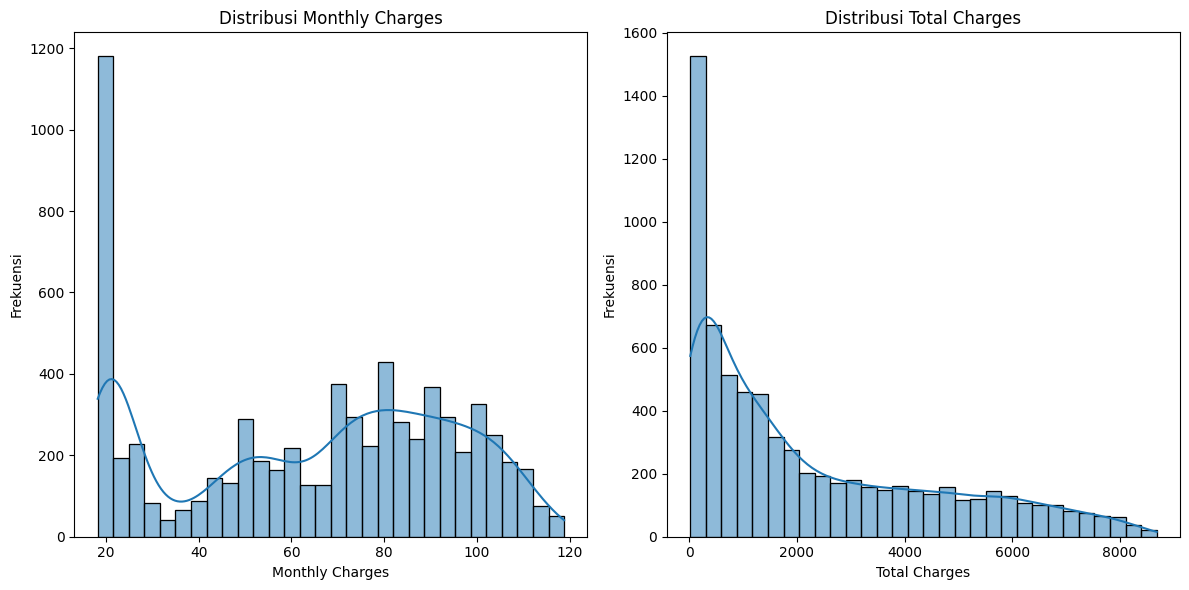
\includegraphics[width=0.8\textwidth]{gambar/histogram.png}
    \caption{Histogram Distribusi Fitur Numerik}
    \label{fig:histogram}
\end{figure}

Dari Gambar \ref{fig:histogram} dapat dilihat bahwa fitur "MonthlyCharges" memiliki distribusi yang cenderung normal, dengan puncak di sekitar nilai 70. Sedangkan fitur "TotalCharges" memiliki distribusi yang cenderung skewed ke kanan, dengan puncak di sekitar nilai 1000. Hal ini menunjukkan bahwa sebagian besar pelanggan memiliki total biaya yang relatif rendah, namun terdapat beberapa pelanggan yang memiliki total biaya yang sangat tinggi.

Selanjutnya kita akan melakukan analisis korelasi antar fitur numerik. Kita akan menggunakan heatmap untuk melihat hubungan antar fitur numerik. Dengan menggunakan .heatmap() dari Seaborn, kita bisa membuat visualisasi yang jelas dan mudah dipahami. Gambar \ref{fig:correlation_heatmap} menunjukkan hasil dari heatmap korelasi antar fitur numerik.

\begin{figure}[H]
    \centering
    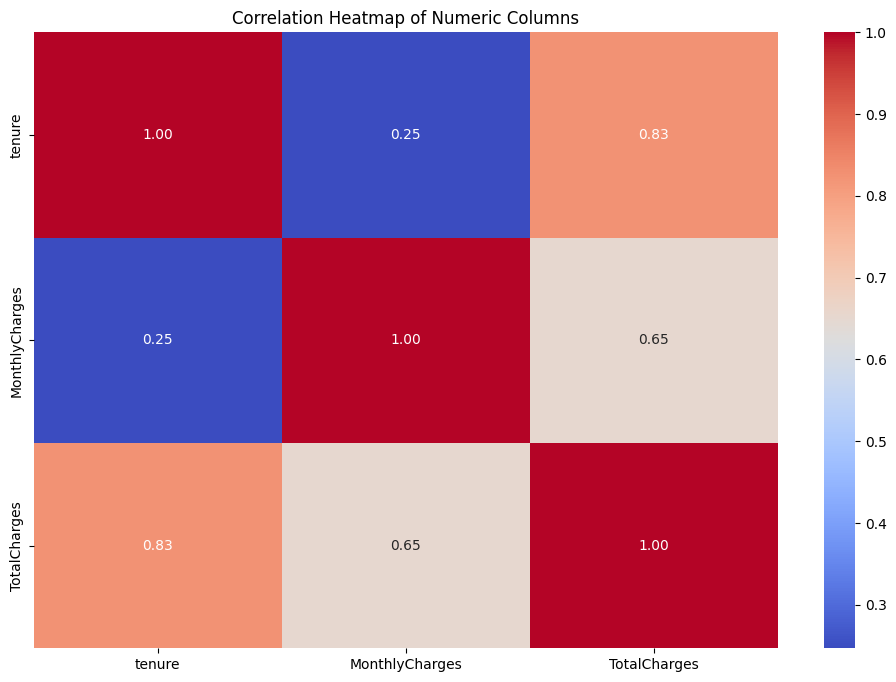
\includegraphics[width=0.8\textwidth]{gambar/heatmapnum.png}
    \caption{Heatmap Korelasi Antar Fitur Numerik}
    \label{fig:correlation_heatmap}
\end{figure}

%jangan masukan fitur tenure pada interpretasi heatmap ini karena sudah binning
Dari Gambar \ref{fig:correlation_heatmap} dapat dilihat bahwa terdapat korelasi yang cukup tinggi antara fitur "MonthlyCharges" dan "TotalCharges", dengan nilai korelasi sekitar 0.65. Hal ini menunjukkan bahwa semakin tinggi biaya bulanan yang dibayarkan oleh pelanggan, semakin tinggi pula total biaya yang dibayarkan selama berlangganan. Sedangkan fitur "tenure" memiliki korelasi yang rendah dengan kedua fitur numerik lainnya, yaitu "MonthlyCharges" dan "TotalCharges".

Kita juga akan melakukan analisis outliers pada fitur-fitur numerik. Kita akan menggunakan boxplot untuk melihat apakah terdapat outliers pada setiap fitur numerik. Dengan menggunakan .boxplot() dari Seaborn, kita bisa membuat visualisasi yang jelas dan mudah dipahami. Gambar \ref{fig:boxplot} menunjukkan hasil dari boxplot outliers pada kedua fitur numerik.

\begin{figure}[H]
    \centering
    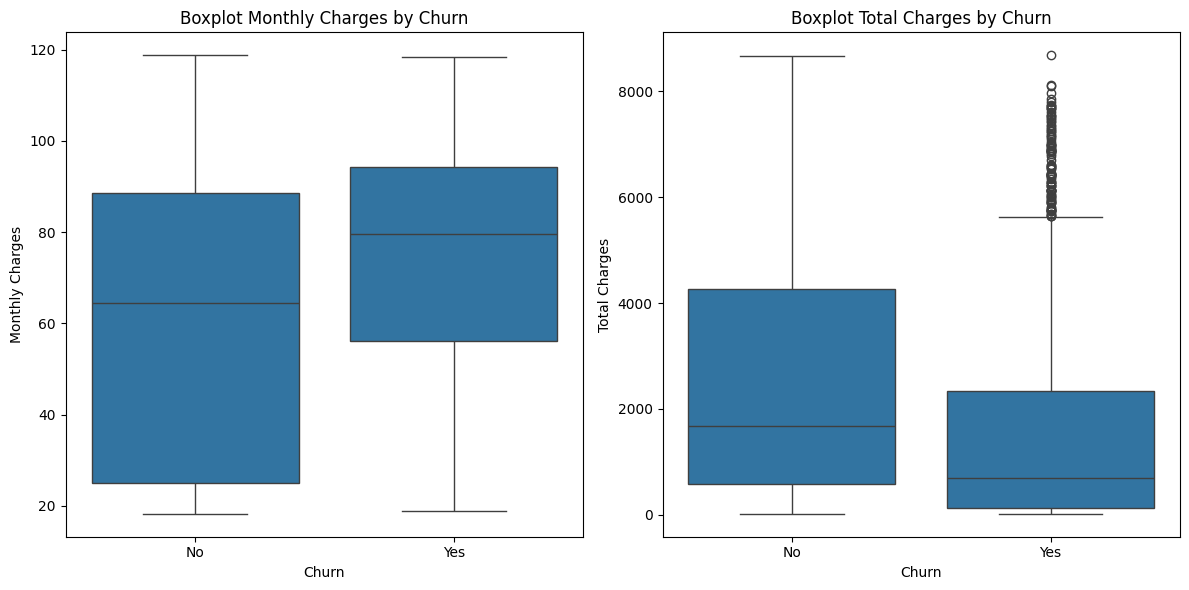
\includegraphics[width=0.8\textwidth]{gambar/boxplot.png}
    \caption{Boxplot Outliers Fitur Numerik}
    \label{fig:boxplot}
\end{figure}

Dari Gambar \ref{fig:boxplot} merupakan boxplot untuk fitur "MonthlyCharges" dan "TotalCharges" berdasarkan kategori "Churn". Dapat dilihat bahwa terdapat beberapa outliers pada kedua fitur numerik tersebut. Outliers ini dapat mempengaruhi hasil analisis dan model yang akan dibangun, sehingga perlu ditangani dengan baik. Kita bisa menghapus outliers tersebut atau menggunakan metode robust scaling untuk mengurangi pengaruh outliers pada model.

Selain itu kita juga mendapatkan bahwa pelanggan dengan biaya bulanan yang lebih tinggi cendrung untuk churn. Hal ini terlihat dari boxplot yang menunjukkan bahwa pelanggan yang churn memiliki biaya bulanan yang lebih tinggi dibandingkan dengan pelanggan yang tidak churn. Sedangkan untuk fitur "TotalCharges", kita tidak bisa menarik kesimpulan yang sama karena terdapat outliers yang cukup signifikan pada kedua kategori dan pada pelanggan yang churn berdasarkan totalcharges cukup datanya cukup tersebar sehingga tidak bisa ditarik kesimpulan yang signifikan.

Setelah melakukan analisis fitur numerik, kita mendapatkan beberapa insight yang dapat digunakan untuk meningkatkan retensi pelanggan. Adapun insight yang didapatkan dari analisis fitur numerik ini adalah sebagai berikut:
\begin{itemize}
    \item Pelanggan dengan lama berlangganan yang lebih lama cenderung memiliki total biaya yang lebih tinggi.
    \item Pelanggan dengan biaya bulanan yang lebih tinggi cenderung memiliki total biaya yang lebih tinggi.
    \item Terdapat segmen highend pada fitur TotalCharges menandakan adanya pelanggan yang memiliki total biaya yang sangat tinggi.
    \item Pelanggan dengan biaya bulanan yang lebih tinggi cenderung untuk churn.
\end{itemize}

Sehingga kita bisa membuat keputusan bisnis yang lebih baik berdasarkan hasil analisis ini. Adapun implikasi bisnisnya dari insight yang dihasilkan adalah sebagai berikut:

\begin{itemize}
    \item Perusahaan dapat mempertimbangkan untuk memberikan penawaran khusus atau promosi kepada pelanggan dengan lama berlangganan yang lebih lama untuk meningkatkan retensi pelanggan.
    \item Perusahaan dapat mempertimbangkan untuk memberikan penawaran khusus atau promosi kepada pelanggan dengan biaya bulanan yang lebih tinggi untuk meningkatkan retensi pelanggan.
    \item Perusahaan dapat mempertimbangkan untuk melakukan segmentasi pelanggan berdasarkan total biaya yang dibayarkan untuk meningkatkan retensi pelanggan.
\end{itemize}

Selain kita juga mendapatkan bahwa fitur tenure yang merupakan fitur numerik yang memiliki informasi tentang lama berlangganan pelanggan, dapat dilakukan binning untuk mengelompokkan pelanggan berdasarkan lama berlangganan mereka. Kita akan membuat 3 kelompok yaitu "0-12 bulan", "13-24 bulan", dan "25+bulan". Maka dengan ini kita bisa melakukan fitur engineering untuk membuat fitur baru yaitu "tenure\_group" yang merupakan hasil binning dari fitur "tenure". Kita akan menggunakan pd.cut() untuk melakukan binning pada fitur "tenure". Dengan begitu kita bisa melihat distribusi pelanggan berdasarkan lama berlangganan mereka.

\subsection{Feature Engineering}
Setelah melakukan analisis terhadap fitur-fitur yang ada dalam dataset, kita akan melakukan feature engineering untuk membuat fitur-fitur baru yang dapat meningkatkan performa model klasifikasi yang akan dibangun. Feature engineering adalah proses menciptakan fitur-fitur baru dari fitur-fitur yang sudah ada untuk meningkatkan kemampuan model dalam memprediksi target variabel.

\subsubsection{Binning Fitur Tenure}
Pada analisa sebelumnya kita mendapatkan bahwa fitur tenure yang merupakan fitur numerik yang memiliki informasi tentang lama berlangganan pelanggan, dapat dilakukan binning untuk mengelompokkan pelanggan berdasarkan lama berlangganan mereka. Kita akan membuat 3 kelompok yaitu "0-12 bulan", "13-24 bulan", dan "25+bulan". Maka dengan ini kita bisa melakukan fitur engineering untuk membuat fitur baru yaitu "tenure\_group" yang merupakan hasil binning dari fitur "tenure". Kita akan menggunakan pd.cut() untuk melakukan binning pada fitur "tenure". Dengan begitu kita bisa melihat distribusi pelanggan berdasarkan lama berlangganan mereka.

\begin{lstlisting}[language=Python, caption=Feature Engineering Binning Fitur Tenure]
# Output setelah binning
tenure_group

oneyear    
threeyear
oneyear  
threeyear
oneyear
\end{lstlisting}

Setelah binning berhasil, selanjutnya saya ingin menguji chi-square untuk melihat apakah fitur tenure\_group ini signifikan terhadap target variabel Churn. Dengan begitu kita bisa mengetahui apakah fitur ini relevan untuk digunakan dalam model klasifikasi.

\begin{lstlisting}[language=Python, caption=Uji Chi-Square Fitur Tenure Group]
# Output uji chi-square
Chi2: 807.5820584283829, p-value: 4.32298939601873e-176, dof: 2
Ada hubungan signifikan antara tenure dan Churn
\end{lstlisting}

Dari hasil uji chi-square di atas, kita mendapatkan nilai Chi2 sebesar 807.58 dengan p-value yang sangat kecil yaitu 4.32e-176. Hal ini menunjukkan bahwa terdapat hubungan yang signifikan antara fitur tenure\_group dan target variabel Churn. Sehingga fitur tenure\_group ini relevan untuk digunakan dalam model klasifikasi.

Selanjutnya saya juga ingin melihat boxplotnya untuk menggali lebih dalam tentang fitur tenure\_group ini. Dengan menggunakan .boxplot() dari Seaborn, kita bisa membuat visualisasi yang jelas dan mudah dipahami. Gambar \ref{fig:tenure_group_boxplot} menunjukkan hasil dari boxplot fitur tenure\_group berdasarkan kategori Churn.

\begin{figure}[H]
    \centering
    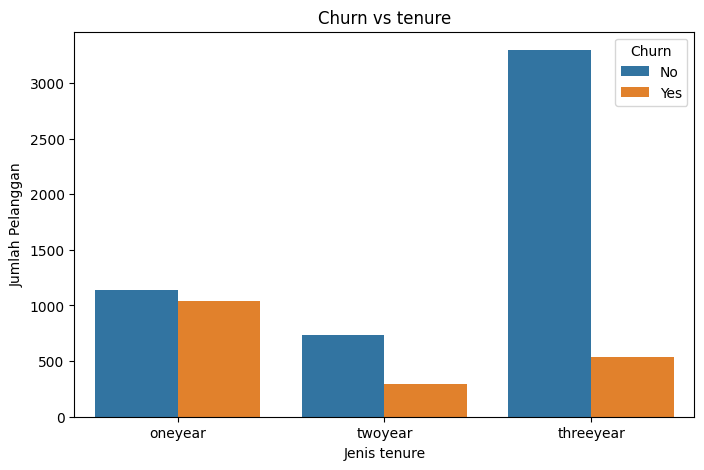
\includegraphics[width=0.8\textwidth]{gambar/tenureboxplot.png}
    \caption{Boxplot Fitur Tenure Group Berdasarkan Kategori Churn}
    \label{fig:tenure_group_boxplot}
\end{figure}

Dari Gambar \ref{fig:tenure_group_boxplot} dapat dilihat bahwa pelanggan yang memiliki lama berlangganan 0-12 bulan cenderung memiliki jumlah churn yang lebih tinggi dibandingkan dengan pelanggan yang memiliki lama berlangganan 13-24 bulan dan 25+bulan. Hal ini menunjukkan bahwa pelanggan yang baru berlangganan cenderung lebih sering berhenti berlangganan dibandingkan dengan pelanggan yang sudah lama berlangganan.

\subsubsection{Binning fitur dengan Uji Chi-Square lemah}
Selain fitur tenure\_group, kita juga akan melakukan binning pada fitur Dependents, partner, dan SeniorCitizen. Saya memutuskan untuk membuat fitur baru bernama is\_married dengan kondisi jika Dependents atau Partner atau SeniorCitizen bernilai "Yes" maka is\_married bernilai "Yes" dan jika tidak maka bernilai "No". Dengan begitu kita bisa melihat distribusi pelanggan berdasarkan status pernikahan mereka.

\begin{lstlisting}[language=Python, caption=Feature Engineering Binning]
# Output setelah binning

    is_married
1    4313
0    2719
Name: count, dtype: int64
\end{lstlisting}

Dengan begitu kita telah berhasil membuat fitur baru bernama is\_married yang merupakan hasil binning dari fitur Dependents, Partner, dan SeniorCitizen.

\subsection{Feature Selection}
Setelah melakukan feature engineering, kita akan melakukan feature selection untuk memilih fitur-fitur yang relevan dan tidak redundant. Feature selection adalah proses memilih fitur-fitur yang paling penting untuk digunakan dalam model klasifikasi. Kita akan menggunakan metode chi-square untuk memilih fitur-fitur yang relevan dengan target variabel Churn.

Pertama tama customerID akan kita buang karena fitur ini tidak relevan untuk digunakan dalam model klasifikasi. Fitur ini hanya berfungsi sebagai identifikasi unik untuk setiap pelanggan dan tidak memberikan informasi yang berguna untuk memprediksi target variabel Churn.

\subsubsection{Berdasarkan Uji Chi-Square}
Kita akan melakukan uji chi-square untuk setiap fitur kategorikal yang ada dalam dataset. Dan telah melakukan feature engineering berdasarkan uji chi-square yang telah dilakukan sebelumnya. Dengan begitu otomatis fitur fitur ini akan dibuang :

\begin{itemize}
    \item Dependents
    \item Partner
    \item SeniorCitizen
    \item tenure
    \item Gender
    \item PhoneService
    \item MultipleLines
    \item TotalCharges
\end{itemize}

Dengan membuang fitur yang tidak relevan, kita akan mendapatkan fitur-fitur yang lebih fokus dan dapat meningkatkan performa model klasifikasi. Adapun fitur-fitur yang akan digunakan dalam model klasifikasi adalah sebagai berikut:

\begin{itemize}
    \item tenure\_group
    \item is\_married
    \item InternetService
    \item OnlineSecurity
    \item OnlineBackup
    \item DeviceProtection
    \item TechSupport
    \item StreamingTV
    \item StreamingMovies
    \item MonthlyCharges
    \item PaperlessBilling
    \item PaymentMethod
    \item Contract
    \item Churn
\end{itemize}

\subsection{Data Preprocessing}
Setelah melakukan feature selection, kita akan melakukan data preprocessing untuk mempersiapkan data sebelum digunakan dalam model klasifikasi. Data preprocessing adalah proses membersihkan dan memformat data agar siap digunakan dalam model klasifikasi. Adapun jenis preprocessing yang akan dilakukan akan tergantung pada jenis data yang ada dalam dataset. Kita akan melakukan preprocessing untuk fitur kategorikal.

\subsubsection{Preprocessing Fitur Kategorikal}
Agar data kategorikal dapat digunakan dalam model klasifikasi, kita perlu mengubah data kategorikal menjadi data numerik. Kita akan menggunakan teknik one-hot encoding untuk mengubah data kategorikal menjadi data numerik. One-hot encoding adalah teknik yang mengubah setiap kategori menjadi kolom baru dengan nilai 0 atau 1. Adapun fitur yang cocok untuk dilakukan one-hot encoding adalah fitur kategorikal yang memiliki lebih dari 2 kategori. Kita akan menggunakan pd.get\_dummies() untuk melakukan one-hot encoding pada fitur kategorikal.
\begin{lstlisting}[language=Python, caption=Preprocessing Fitur Kategorikal]
# Preprocessing fitur kategorikal setelah data di split

X_train = pd.get_dummies(X_train, columns=['tenure_group', 'is_
married', 'InternetService', 'OnlineSecurity',
 'OnlineBackup', 'DeviceProtection', 'TechSupport'
 , 'StreamingTV', 'StreamingMovies', 'PaperlessBill
ing', 'PaymentMethod', 'Contract'], drop_first=True)

X_test = pd.get_dummies(X_test, columns=['tenure_group', 
'is_married', 'InternetService', 'OnlineSecurity',
 'OnlineBackup', 'DeviceProtection', 'TechSupport',
  'StreamingTV', 'StreamingMovies', 'PaperlessBilling',
   'PaymentMethod', 'Contract'], drop_first=True)

# Menyelaraskan kolom pada X_test dengan X_train
X_test = X_test.reindex(columns=X_train.columns, fill_value=0)
\end{lstlisting}

Setelah melakukan one-hot encoding, kita akan mendapatkan fitur-fitur baru yang merupakan hasil dari one-hot encoding. Adapun untuk fitur fitur yang hanya terdiri dari 2 kategori seperti is\_married, kita akan mengubahnya menjadi 0 dan 1. Fitur ini akan diubah menjadi numerik dengan cara mengubah nilai "Yes" menjadi 1 dan "No" menjadi 0. Dengan begitu kita akan mendapatkan fitur-fitur yang siap digunakan dalam model klasifikasi. Gambar \ref{fig:one_hot_encoding} menunjukkan hasil dari preprocessing pada fitur kategorikal.

\begin{figure}[H]
    \centering
    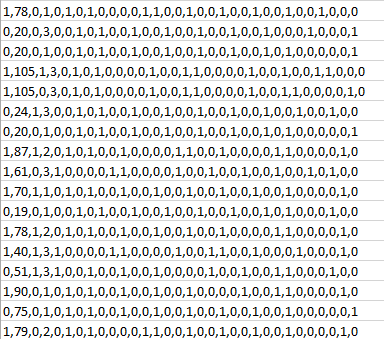
\includegraphics[width=0.4\textwidth]{gambar/onehotencoding.png}
    \caption{Hasil One-Hot Encoding Fitur Kategorikal}
    \label{fig:one_hot_encoding}
\end{figure}

Setelah melakukan preprocessing pada fitur kategorikal, kita akan mendapatkan data yang siap digunakan dalam model klasifikasi. Namun sebelum itu kita juga perlu melakukan preprocessing pada fitur numerik.

\newpage
\subsubsection{Preprocessing Fitur Numerik}
Untuk fitur numerik, kita hanya memiliki 1 fitur yang perlu dilakukan preprocessing yaitu fitur MonthlyCharges. Namun karena ini adalah satu satunya fitur numerik yang ada dalam dataset, saya memutuskan untuk tidak melakukan preprocessing pada fitur ini. Kita akan menggunakan fitur ini apa adanya tanpa melakukan scaling atau normalisasi. Hal ini karena fitur ini merupakan satu satunya fitur numerik sehingga tidak ada fitur lain yang perlu diselaraskan dengan fitur ini. 

Selain itu kita juga tidak perlu melakukan transformasi log pada fitur ini karena fitur ini sudah memiliki distribusi yang cenderung normal. Sehingga kita akan menggunakan fitur MonthlyCharges apa adanya tanpa melakukan preprocessing.

Setelah semua siap kita akan lanjut ke tahap selanjutnya yaitu membangun model klasifikasi. Kita akan menggunakan model klasifikasi yang sudah umum digunakan seperti Logistic Regression, Decision Tree, Random Forest, dan XGBoost. Kita akan membandingkan performa dari setiap model untuk memilih model yang terbaik.

\subsection{Handling Imbalanced Data}
Setelah melakukan preprocessing pada data, kita akan melakukan handling imbalanced data. Imbalanced data adalah kondisi di mana jumlah data pada setiap kelas tidak seimbang. Hal ini dapat mempengaruhi performa model klasifikasi yang akan dibangun. Namun pertama tama kita akan melakukan analisis terhadap distribusi kelas pada target variabel Churn. Kita akan menggunakan .value\_counts() untuk melihat distribusi kelas pada target variabel Churn.

\begin{lstlisting}[language=Python, caption=Distribusi Kelas pada Target Variabel Churn]
# Distribusi kelas pada target variabel Churn
Kelas 0: 4130 sampel
Kelas 1: 1495 sampel
\end{lstlisting}

Dari hasil distribusi kelas pada target variabel Churn, kita mendapatkan bahwa jumlah sampel pada kelas 0 (tidak churn) jauh lebih banyak dibandingkan dengan kelas 1 (churn). Hal ini menunjukkan bahwa data yang kita miliki tidak seimbang.

Namun jika dihitung dari rasionya  jumlah kelas 0 (tidak churn) adalah sekitar 73.8\% dan jumlah kelas 1 (churn) adalah sekitar 26.2\%. Hal ini menunjukkan bahwa data yang kita miliki masih dalam batas wajar untuk digunakan dalam model klasifikasi. Sehingga kita tetap perlu melakukan tuning pada model dengan menambahkan class\_weight='balanced' pada setiap model yang akan kita gunakan. Dengan begitu model akan memberikan bobot yang lebih besar pada kelas yang kurang terwakili yaitu kelas 1 (churn).

\newpage

